\documentclass[10pt]{beamer}

\usepackage{bbold}
\usepackage{pst-plot}
\usepackage{amsmath}
\usepackage{amssymb}
\usepackage{algorithm}
\usepackage{algorithmic}
\usepackage{verbatim}

\usepackage[utf8]{inputenc}
\usepackage{default}

\floatname{algorithm}{Algorithme}
\renewcommand{\algorithmicrequire}{\textbf{Entr\'{e}e(s)}}
\renewcommand{\algorithmicensure}{\textbf{Sortie(s)}}
\renewcommand{\algorithmicdo}{\textbf{faire}}
\renewcommand{\algorithmicendwhile}{\textbf{fin du tant que}}
\renewcommand{\algorithmicend}{\textbf{fin}}
\renewcommand{\algorithmicif}{\textbf{si}}
\renewcommand{\algorithmicendif}{\textbf{fin du si}}
\renewcommand{\algorithmicelse}{\textbf{sinon}}
\renewcommand{\algorithmicelsif}{\textbf{fin du sinon}}
\renewcommand{\algorithmicthen}{\textbf{alors}}
\renewcommand{\algorithmicfor}{\textbf{pour}}
\renewcommand{\algorithmicforall}{\textbf{pour tout}}
\renewcommand{\algorithmicto}{\textbf{\`{a}}}
\renewcommand{\algorithmicendfor}{\textbf{fin du pour}}
\renewcommand{\algorithmicdo}{\textbf{faire}}
\renewcommand{\algorithmicloop}{\textbf{boucler}}
\renewcommand{\algorithmicendloop}{\textbf{fin de la boucle}}
\renewcommand{\algorithmicrepeat}{\textbf{répéter}}
\renewcommand{\algorithmicuntil}{\textbf{jusqu’à}}
\renewcommand{\algorithmicprint}{\textbf{afficher}}

\definecolor{blue}{rgb}{0,0,.750}
\definecolor{green}{rgb}{0,.750,0}
\definecolor{red}{rgb}{.750,0,0}
\definecolor{orange}{rgb}{.932,.464,0}

\beamerboxesdeclarecolorscheme{def}{blue}{blue!10}
\beamerboxesdeclarecolorscheme{ex}{green}{green!10}
\beamerboxesdeclarecolorscheme{theorem}{red}{red!10}
\beamerboxesdeclarecolorscheme{prop}{orange}{orange!10}

\addtobeamertemplate{navigation symbols}{}{%
    \hspace{1em}%
    \insertframenumber/\inserttotalframenumber
}

\title[Compression par ondelettes]{Compression d'images par ondelettes}
\author{Benjamin CATINAUD}
\date{Ann\'{e}e 2017 - 2018}

\usetheme{Copenhagen}

\begin{document}

  \frame{\titlepage}
  
  \begin{frame}
   \centering
   \textbf{\LARGE Introduction}
   
   \begin{itemize}
    \item Plus de 2200 photos mises en ligne sur Facebook par seconde\footnote{\tiny Source : \textit{www.planetoscope.com}}
    \item D\'{e}bit moyen en France : 8.9 Mbps
    \item Taille d'une image : de l'ordre du m\'{e}gaoctet
   \end{itemize}

  \end{frame}

  
  \begin{frame}
    \tableofcontents
  \end{frame}
  
  \section{Th\'{e}orie des ondelettes}
  
    \subsection{Une ondelette, c'est quoi ?}
    
      \begin{frame}
	\begin{beamerboxesrounded}[scheme=def]{D\'{e}finition : Ondelette}
	  \begin{itemize}
	  \item Fonction $\psi$ de carr\'{e} int\'{e}grable sur $\mathbb{R}$ $\Big( \int_{\mathbb{R}} \mid \psi \mid^2 \, < \, + \infty \Big)$
	  \item Support de $\psi$ compact
	  \item $\int_{\mathbb{R}} \psi$ converge et vaut $0$
	  \item Cr\'{e}ation d'une famille d'ondelettes par dilatation et translation de l'ondelette m\`{e}re 
	    $\Big(\psi_{a,b}(t) = \psi \big( \frac{t - b}{a} \big) \Big)$
	  \end{itemize}
	\end{beamerboxesrounded}
	
	\begin{beamerboxesrounded}[scheme=ex]{Exemples : Ondelette de Daubechies et de Haar}
	    
	  \begin{figure}[!h]
	    \begin{tabular}{cc}
	      
	      \hspace{-3cm}{
	      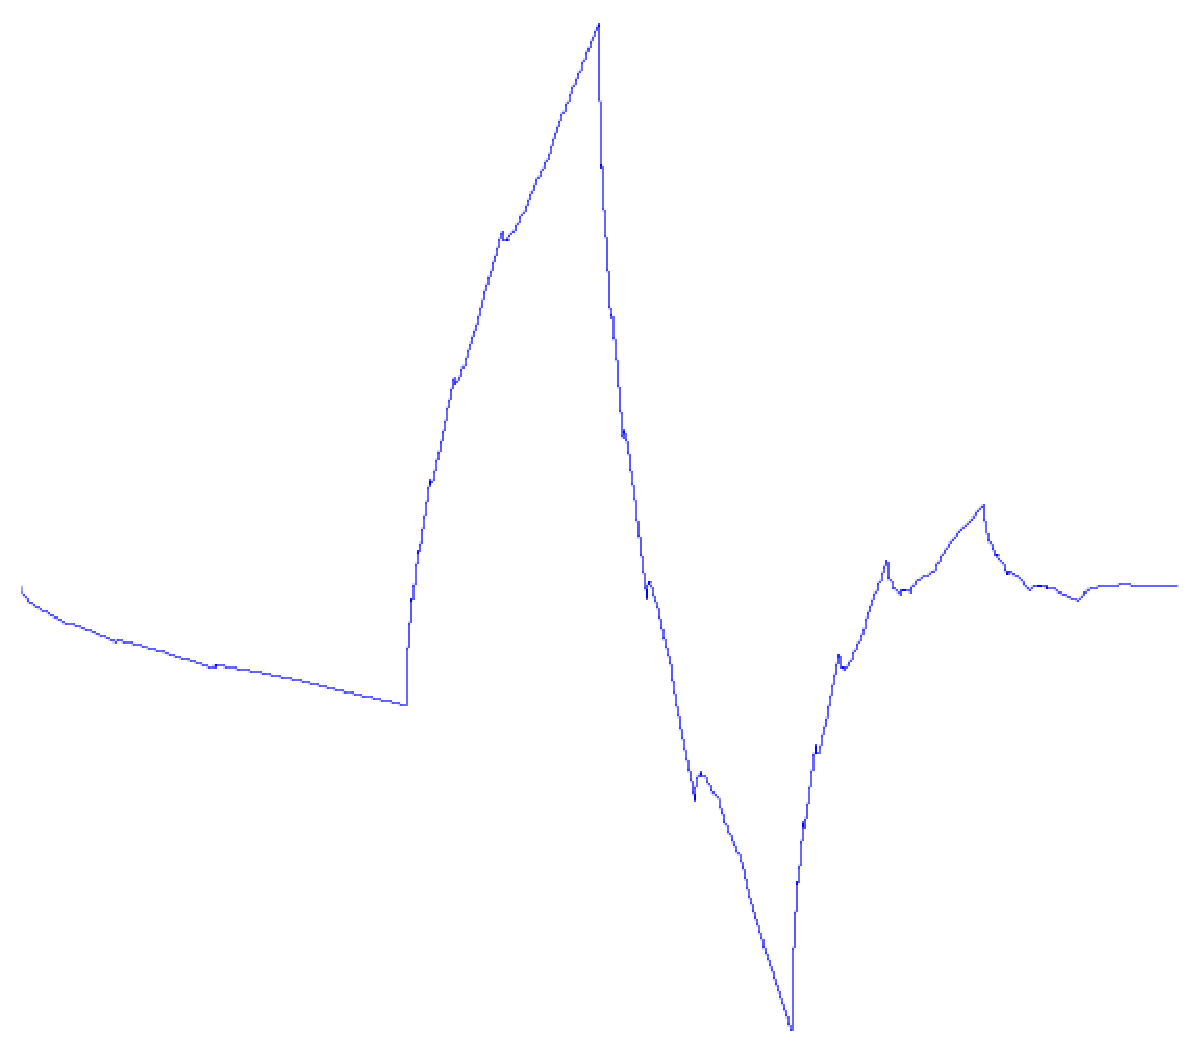
\includegraphics[width = 0.3 \linewidth]{daubechies.eps}
	      } \hspace{1cm} &
	    
	      \begin{pspicture}(-0.2,-1.5)(1.5,1.5)
		\psset{algebraic=true}
		\psset{xunit = 3cm, yunit = 1cm}
		\psaxes{->}(0,0)(-0.2,-1.5)(1.5,1.5)
		\psplot{0}{0.5}{1}
		\psline[linestyle=dotted](0.5,1)(0.5,-1)
		\psplot{0.5}{1}{-1}
		\psline[linestyle=dotted](1,-1)(1,0)
	      \end{pspicture} \\
	      
	    \end{tabular}         
	  \end{figure}
	  
	\end{beamerboxesrounded}

      \end{frame}
  
    \subsection{Analyse multi-r\'{e}solution - Espaces d'approximation}
    
      \begin{frame}
      
	\textbf{Analyse multi-r\'{e}solution : Espaces d'approximation}
	
	\begin{beamerboxesrounded}[scheme=def]{D\'{e}finition}
	  Soit $j \in \mathbb{Z}$. \textbf{Espace d'aproximation \`{a} l'\'{e}chelle $ 2 ^ j $} : 
	  espace vectoriel $V_j$ des fonctions de $ L^2(\mathbb{R}, \mathbb{R}) $ constantes sur
	  les intervalles de la forme $ [2^j k; 2^j (k \, + \, 1)[, \; k \; \in \; \mathbb{Z}$
	\end{beamerboxesrounded}
	  
	\begin{beamerboxesrounded}[scheme=theorem]{Propri\'{e}t\'{e}s fondamentales}
	  \begin{itemize}
	    \item $ \forall j \in \mathbb{Z}, V_{j + 1} \subseteq V_j $
	    \item $ \displaystyle \bigcup_{j \in \mathbb{Z}} V_j $ est dense dans $ L^2(\mathbb{R}, \mathbb{R}) $ \\
	  \end{itemize}
	\end{beamerboxesrounded}
	    
	\begin{beamerboxesrounded}[scheme=prop]{Caract\'{e}risation}
	  \begin{center}
	      $ \forall j \in \mathbb{Z}, V_j \; = \; 
	      \Bigg< \Big\{ \phi_{j,k} = \frac{1}{\sqrt{2^j}} \mathbb{1}_{[2^j k; 2^j (k \, + \, 1)[}, \; k \in \mathbb{Z} \Big\} \Bigg> $ 
	  \end{center}
	\end{beamerboxesrounded}
	
      \end{frame}
      
    \subsection{Analyse multi-r\'{e}solution - Espaces de d\'{e}tails}

      \begin{frame}
	
	\textbf{Analyse multi-r\'{e}solution}
	
	\begin{beamerboxesrounded}[scheme=def]{D\'{e}finition des espaces de d\'{e}tails}
	  On d\'{e}finit $ W_j , $ pour $ j \, \in \, \mathbb{Z} $, tel que 
	  \begin{center}
	    \vspace{-0.4cm}
	    $ V_{j - 1} \, = \, V_j \displaystyle \bigoplus^\perp W_j $
	  \end{center}
	\end{beamerboxesrounded}
	
	\begin{beamerboxesrounded}[scheme=prop]{Caract\'{e}risation des espaces de d\'{e}tails}
	    \centering
	    $\forall j \in \mathbb{Z}, W_j \; = \; $ \\ $
	    \Bigg< \Big\{ \psi_{j,k} \; = \; \frac{1}{\sqrt{2^j}} \big(\mathbb{1}_{[2^{j - 1} k ; 2^{j - 1} (k + 1)[} - 
		\mathbb{1}_{[2^{j - 1} (k + 1) ; 2^{j - 1} (k + 2)[} \big),  \; k \in \mathbb{Z} \Big\} \Bigg>$ 
	\end{beamerboxesrounded}
	
	\begin{beamerboxesrounded}[scheme=prop]{Propri\'{e}t\'{e} des fonctions g\'{e}n\'{e}ratrices}
	  On remarque la relation de r\'{e}currence :
	    \begin{center}
	      $ \phi_{j,k} = \frac{1}{\sqrt{2}} (\phi_{j - 1, 2 k} + \phi_{j - 1, 2 k + 1}) $ \\
	      $ \psi_{j,k} = \frac{1}{\sqrt{2}} (\phi_{j - 1, 2 k} - \phi_{j - 1, 2 k + 1}) $
	    \end{center}
	\end{beamerboxesrounded}
	
      \end{frame}
      
  \section{Algorithme de Mallat}
  
    \subsection{D\'{e}finitions}
  
      \begin{frame}
	\begin{beamerboxesrounded}[scheme=def]{D\'{e}finition : Vecteurs associ\'{e}s \`{a} la transformation par ondelettes de Haar}
	  \begin{center}
	    $ \mathcal{H}_a \; = \; \frac{1}{2} (1, 1) \; \in \; \mathbb{R}^2 $ pour les espaces $(V_j)_{j \in \mathbb{Z}}$ \\
	    $ \mathcal{H}_d \; = \; \frac{1}{2} (1, -1) \; \in \; \mathbb{R}^2 $ pour les espaces $(W_j)_{j \in \mathbb{Z}}$
	  \end{center}
	\end{beamerboxesrounded}
	  
	\begin{beamerboxesrounded}[scheme=def]{D\'{e}finition : Fonction filtre}
	    Pour $ b, x \in \mathbb{R}^n $ et $ a \in \mathbb{R}^* $, 
	    la fonction filtre $ \Phi_{a,b} $ est telle que
	    \begin{center}
	      $ \forall i \in [1;n], \; \Big(\Phi_{a,b}(x)\Big)_k \; = \; \frac{1}{a} \displaystyle\sum_{i = 1}^k b_i x_{k - i} $
	    \end{center}
	    On notera $\varPhi$ la fonction filtre sur les espaces d'approximation
	    et $\varPsi$ celle sur les espaces de d\'{e}tails 
	\end{beamerboxesrounded}
	    
	\begin{beamerboxesrounded}[scheme=def]{D\'{e}finition : Fonction d'\'{e}chantillonage}
	    \begin{center}
	      $ \downarrow_2 \, : \mathbb{R}^n \longrightarrow \mathbb{R}^{\lfloor n / 2 \rfloor} $ \\
	      $ (x_1, x_2, ..., x_n) \longmapsto (x_2, x_{4}, ..., x_{2 \lfloor n / 2 \rfloor}) $
	    \end{center}
	\end{beamerboxesrounded}
	
      \end{frame}
      
    \subsection{Algorithme de transformation $WT$}
      
      \begin{frame}
	\begin{algorithm}[H]
	  \caption{Transform\'{e}e par ondelettes d'une matrice}
	  
	  \begin{algorithmic}
	    \REQUIRE { une matrice $M \in M_{n,m}(\mathbb{R}) $ et un entier $j_V \in \mathbb{N}$ }
	    \STATE {Normaliser $M$}
	    
	    \FOR { $k = 0$ \TO $j_V - 1$}
	      \FOR { $i = 1$ \TO $n / 2^k$}
		\STATE { Affecter au vecteur $M_{i,[1;\frac{m}{2^{k + 1}}]}$ le r\'{e}sultat de
		  $ (\downarrow_2 \, $o$ \, \varPhi) \Big(M_{i,[1;\frac{m}{2^k}]}\Big)$ }
		\STATE { Affecter au vecteur $M_{i,[\frac{m}{2^{k + 1}} + 1;\frac{m}{2^k}]}$ le r\'{e}sultat de
		  $ (\downarrow_2 \, $o$ \, \varPsi) \Big( M_{i,[1;\frac{m}{2^k}]} \Big)$  }
	      \ENDFOR
	      \FOR { $j = 1$ \TO $m / 2^k$}
		\STATE { Affecter au vecteur $M_{[1;\frac{n}{2^{k + 1}}],j}$ le r\'{e}sultat de
		  $ (\downarrow_2 \, $o$ \, \varPhi) \Big( M_{[1;\frac{n}{2^k}],j} \Big) $ }
		\STATE { Affecter au vecteur $M_{[\frac{n}{2^{k + 1}} + 1;\frac{n}{2^k}],j}$ le r\'{e}sultat de
		  $ (\downarrow_2 \, $o$ \, \varPsi) \Big( M_{[1;\frac{n}{2^k}],j} \Big)$  }
	      \ENDFOR
	    \ENDFOR
	    \ENSURE {La matrice $M$ ainsi obtenue}
	  \end{algorithmic}

	\end{algorithm}
	
      \end{frame}
      
    \subsection{Algorithme de reconstruction $WR$}
      
      \begin{frame}
	\begin{algorithm}[H]
	  \caption{Reconstruction d'une matrice}
	  
	  \begin{algorithmic}
	    \REQUIRE { une matrice $M \in M_{n,m}(\mathbb{R}) $ et un entier $j_V \in \mathbb{N}$ }	
	    \FOR { $k = j_V - 1$ \TO $0$}
	      \FOR { $j = 1$ \TO $m / 2^k$}
		\STATE { Affecter au vecteur $M_{[1;\frac{n}{2^k}],j}$ la somme de
		  $ (\varGamma \, $o$ \, \uparrow_2) \Big( M_{[1;\frac{n}{2^{k + 1}}],j} \Big) $ \\ et de
		  $(\varOmega \, $o$ \, \uparrow_2) \Big( M_{[\frac{n}{2^{k + 1}} + 1;\frac{n}{2^k}],j} \Big)$ }
	      \ENDFOR
	      \FOR { $i = 1$ \TO $n / 2^k$}
		\STATE { Affecter au vecteur $M_{i,[1;\frac{m}{2^{k}}]}$  la somme de 
		    $ (\varGamma \, $o$ \, \uparrow_2) \Big( M_{i,[1;\frac{m}{2^{k + 1}}]} \Big) $ 
		    et de $ (\varOmega \, $o$ \, \uparrow_2) \Big( M_{i,[\frac{m}{2^{k + 1}} + 1;\frac{m}{2^k}]} \Big)$ }
	      \ENDFOR
	    \ENDFOR
	    \ENSURE {La matrice $M$ ainsi obtenue}
	  \end{algorithmic}

	\end{algorithm}
      \end{frame}
      
    \subsection{Et concr\`{e}tement ?}

      \begin{frame}
	\begin{figure}[H]
	  \centering
	  \begin{tabular}{cc}
	    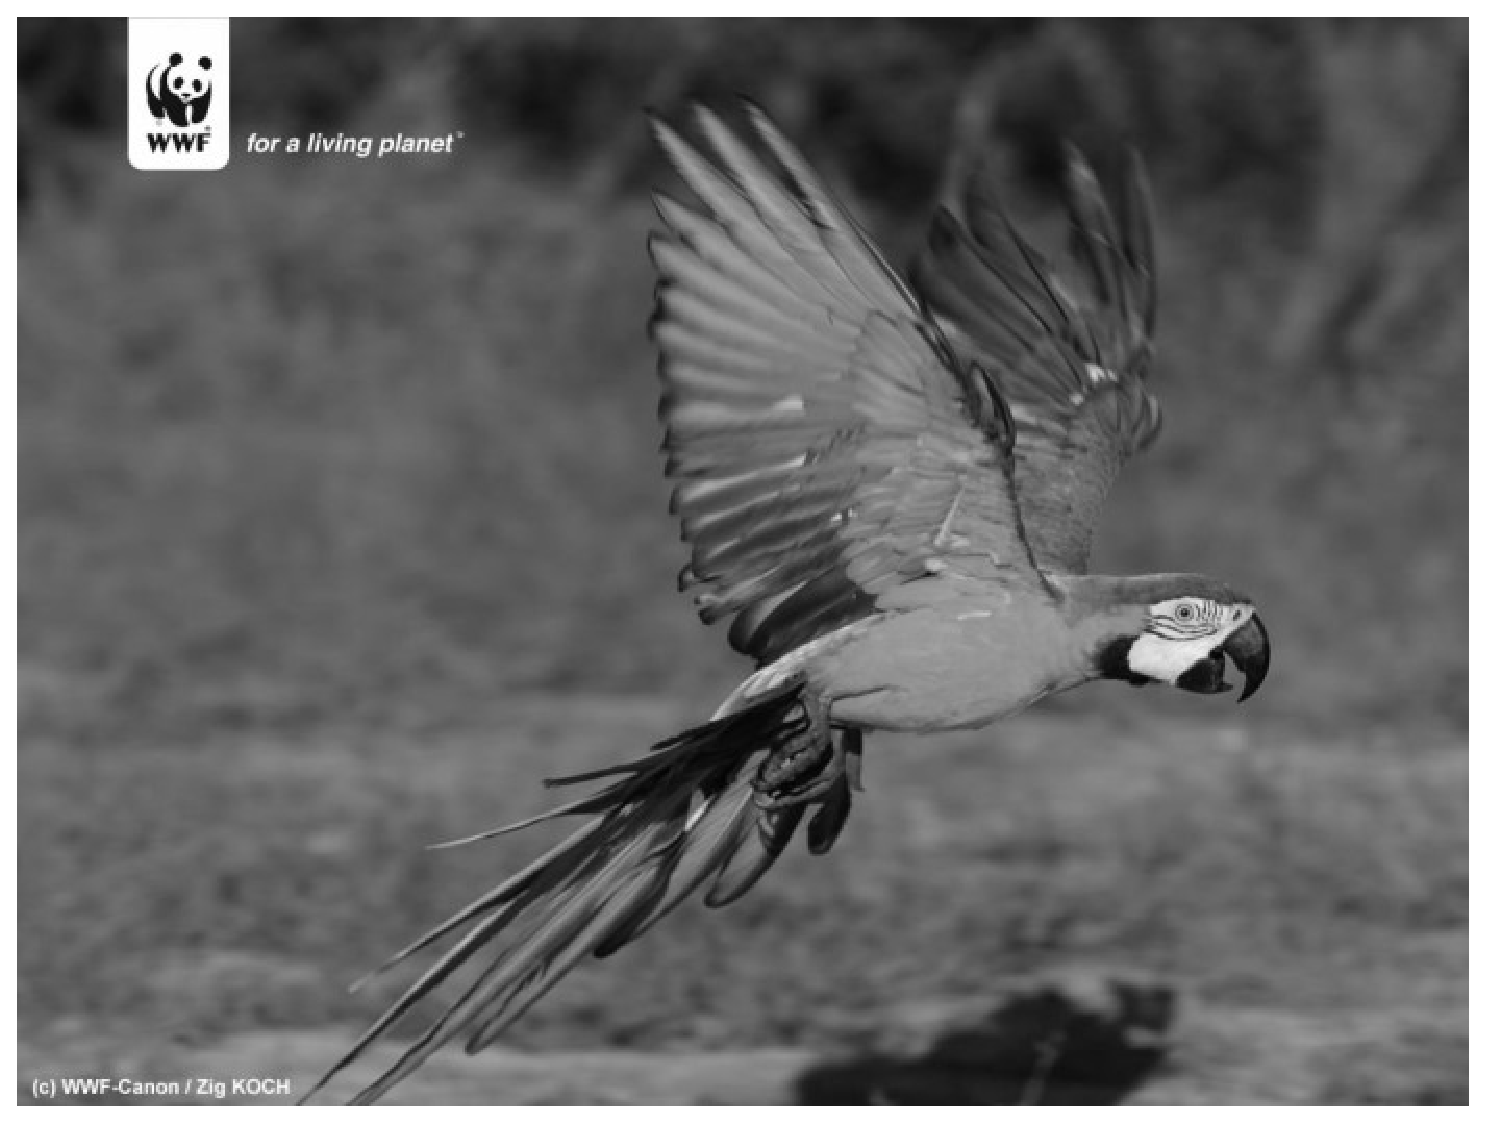
\includegraphics[width = 0.4 \linewidth]{ara_orig.eps} &
	    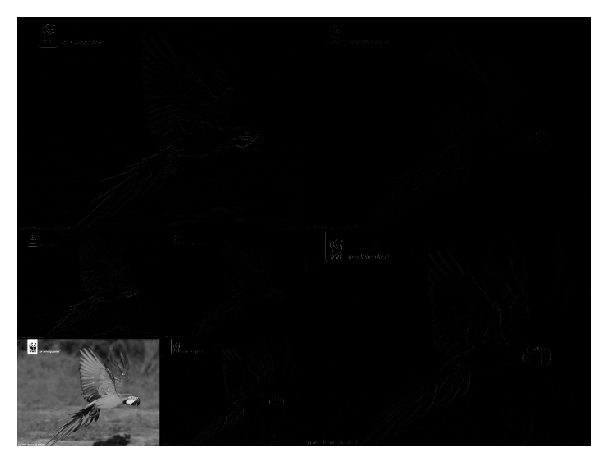
\includegraphics[width = 0.4 \linewidth]{ara_wt_V1.eps} 
	  \end{tabular}
	  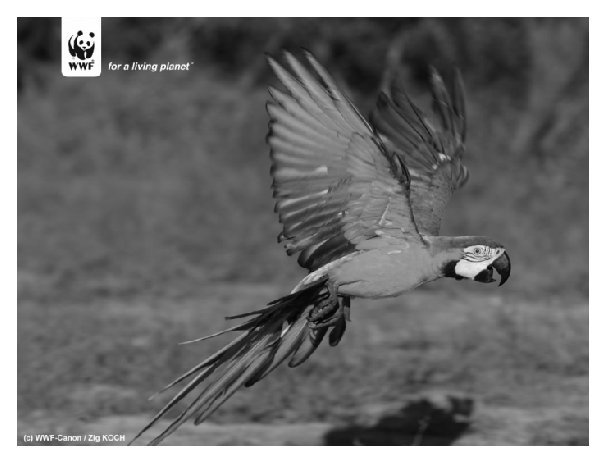
\includegraphics[width = 0.4 \linewidth]{ara_decomp.eps}
	\end{figure}   

      \end{frame}
      
  \section{Un algorithme efficace ?}
  
    \subsection{Complexit\'{e}}
      
      \begin{frame}
	\begin{beamerboxesrounded}[scheme=prop]{Complexit\'{e} de la fonction $WT$}
	  Pour une image de taille $n$x$m$ pixels, on a une complexit\'{e} de :
	  \begin{center}
	    $ \boxed{O \Big(nm + n m^2 + m n^2 \Big) \; = \; O \Big( \big(\max(n,m)\big)^3 \Big)} $
	  \end{center}
	\end{beamerboxesrounded}
	  
	\begin{figure}[H]
	    \centering
	    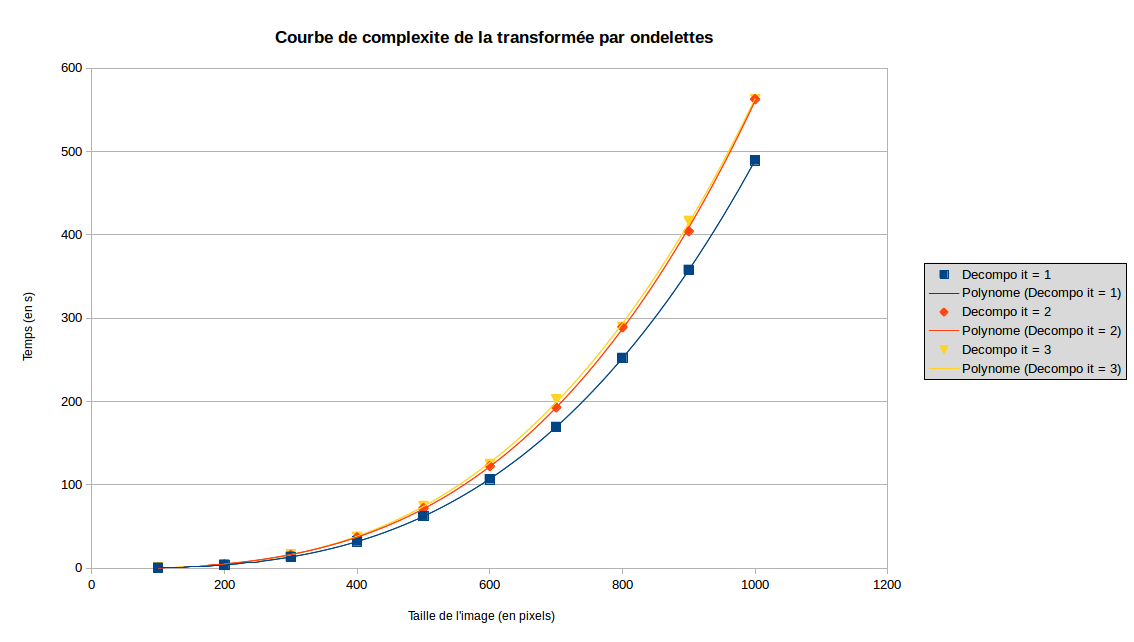
\includegraphics[width = 0.8 \linewidth]{complexite_decompo.eps}
	\end{figure}
      \end{frame}
    
    \subsection{Taux de compression}

      \begin{frame}
	\begin{figure}[!h]
	    \centering
	    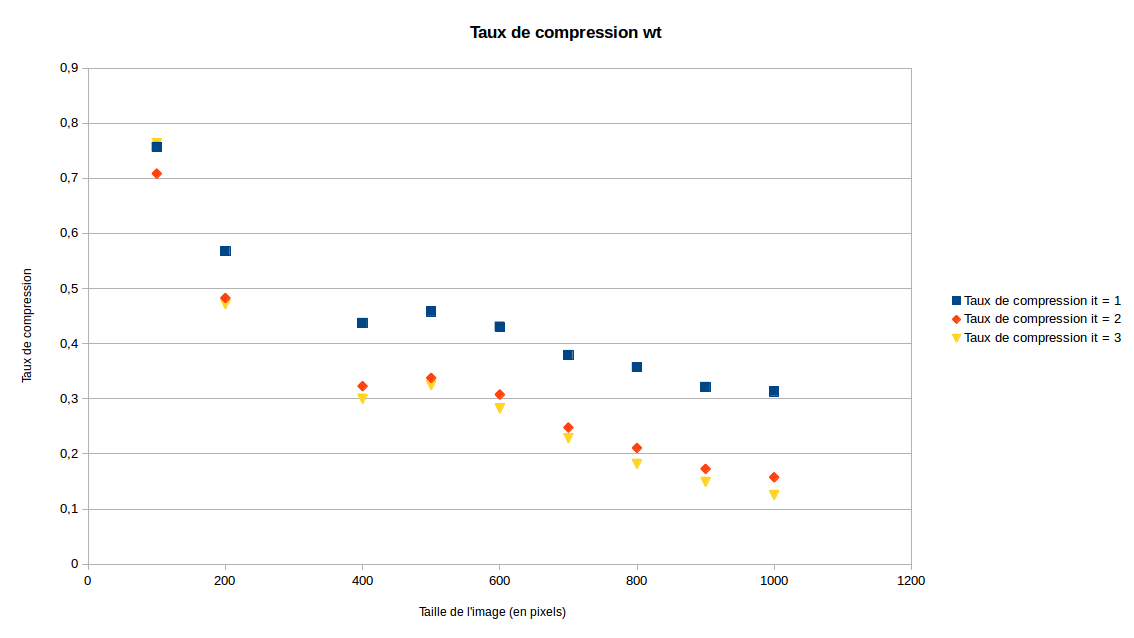
\includegraphics[width = 0.9 \linewidth]{taux_compression.eps}
	\end{figure}
      \end{frame}
    
    \subsection{Estimation de l'erreur}

      \begin{frame}
	\begin{beamerboxesrounded}[scheme=prop]{Distance de compression}
	  On peut d\'{e}finir une distance de la mani\`{e}re suivante :
	  \begin{center}
	    $d : M_{n,m}(\mathbb{R}) \, $x$ \, M_{n,m}(\mathbb{R}) \longrightarrow \mathbb{R}^+ $ \\
	    $ (M, N) \longmapsto \frac{\parallel M - N \parallel}{n m} $
	  \end{center}
	\end{beamerboxesrounded}

	\begin{beamerboxesrounded}[scheme=def]{D\'{e}finition : Fonction erreur}
	  On d\'{e}finit la fonction erreur pour $j_V \in \mathbb{N}$ comme suit avec $\gamma_{j_V}$ la fonction de compression 
	    et $\rho_{j_V}$ la fonction de d\'{e}compression :
	  \begin{center}
	    $\mathcal{E}_{j_V} : M_{n,m}(\mathbb{R}) \longrightarrow \mathbb{R}  $ \\
	    $M \longmapsto d \Bigg(M, \Big(\rho_{j_V} \, $o$ \, \gamma_{j_V}\Big)(M) \Bigg)$
	  \end{center}
	\end{beamerboxesrounded}
	
      \end{frame}
      
      \begin{frame}
	\begin{figure}[!h]
	    \centering
	    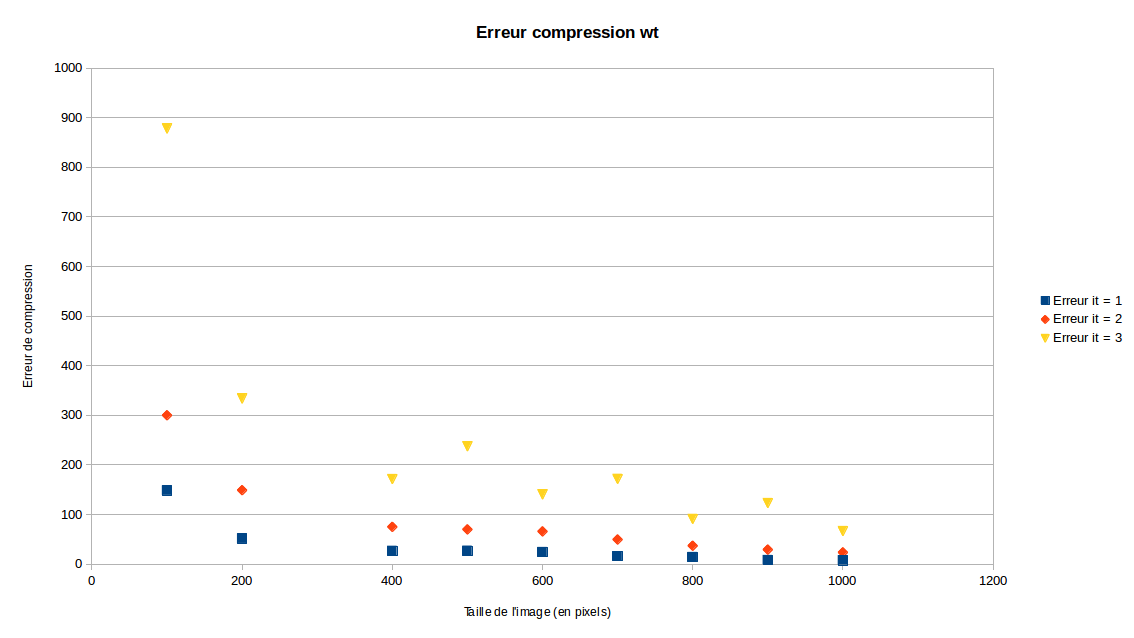
\includegraphics[width = 0.9 \linewidth]{erreur_compression.eps}
	\end{figure}	
      \end{frame}

      
  \section{Bilan visuel}
      
    \begin{frame}      
      \begin{figure}[H]
	\centering
	\begin{tabular}{cc}
	  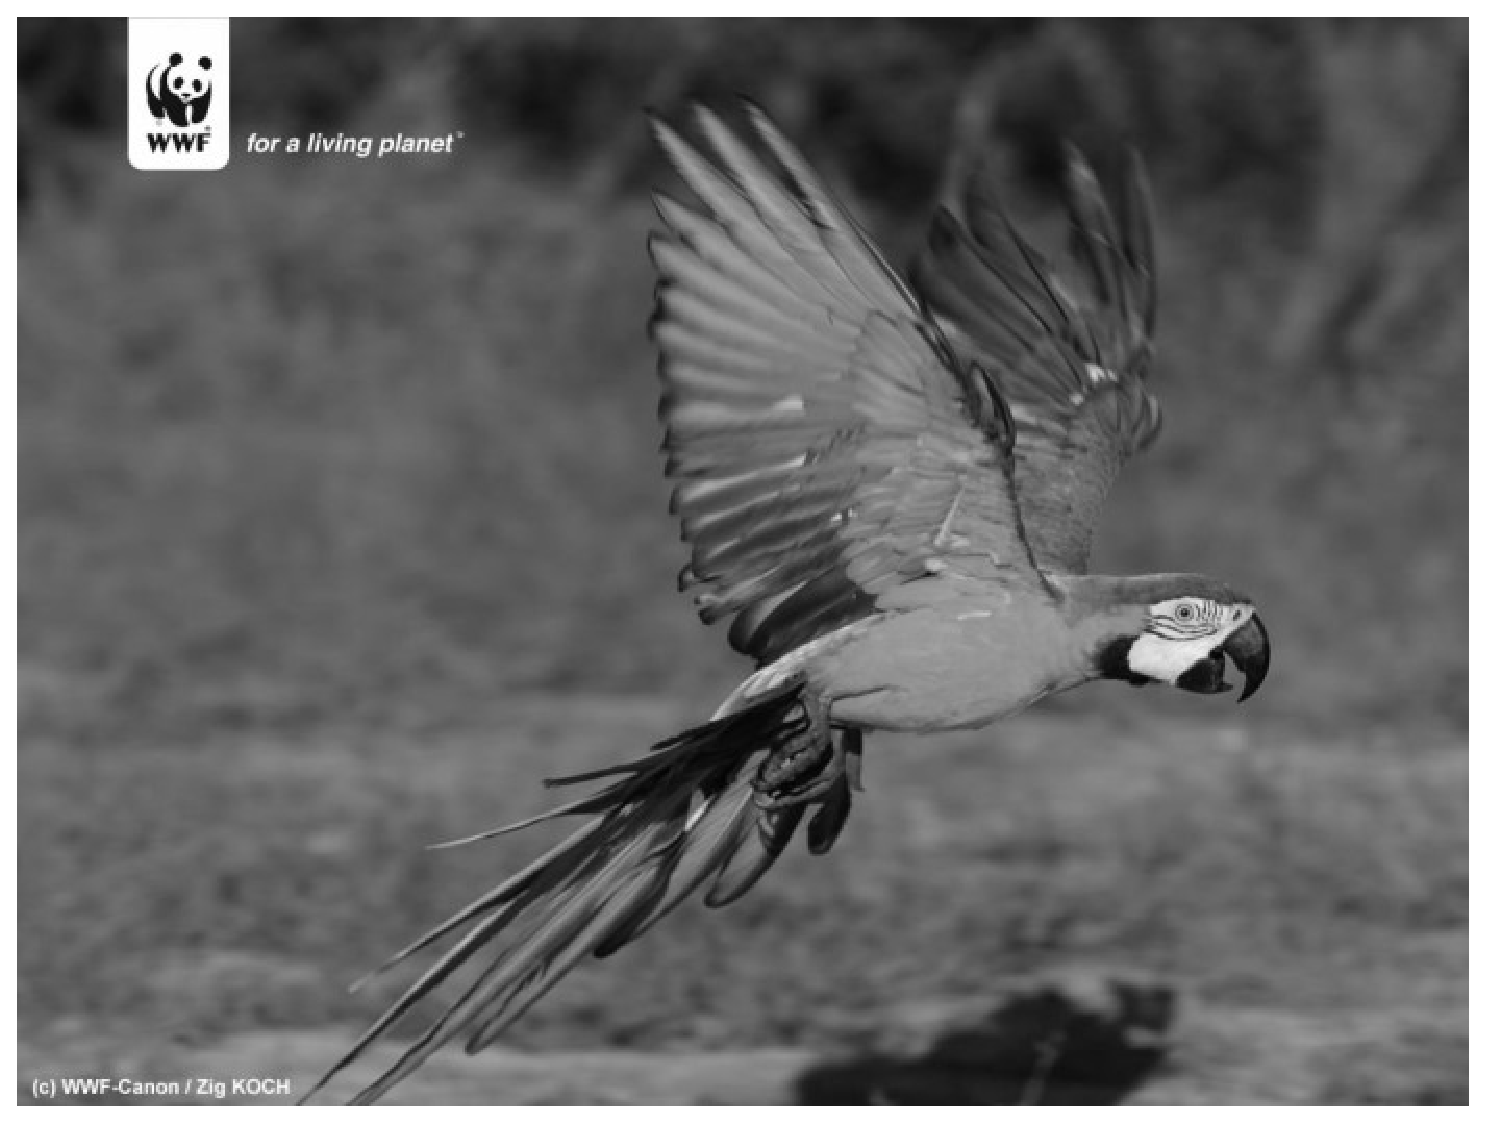
\includegraphics[width = 0.45 \linewidth]{ara_orig.eps} &
	  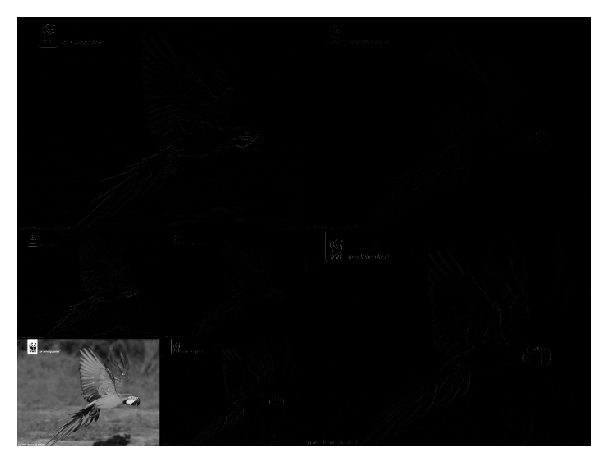
\includegraphics[width = 0.45 \linewidth]{ara_wt_V1.eps} \\
	  
	  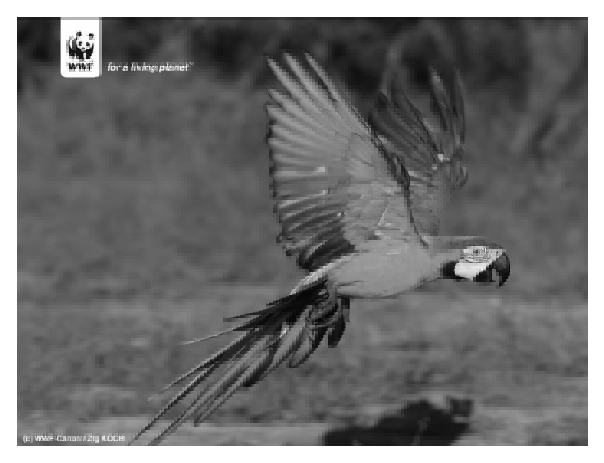
\includegraphics[width = 0.45 \linewidth]{decomp_ara.eps} &
	  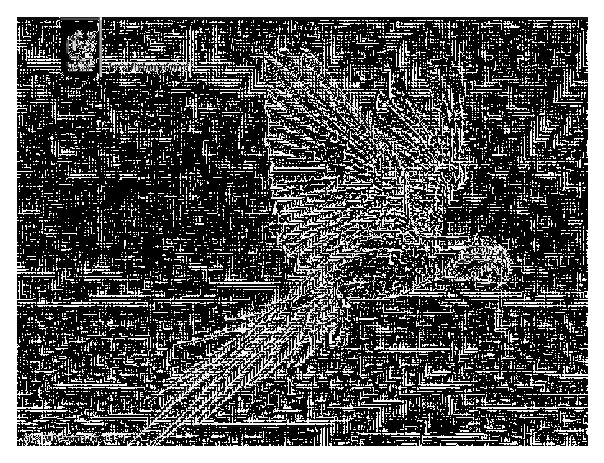
\includegraphics[width = 0.45 \linewidth]{error_ara.eps} \\	
	\end{tabular}
      \end{figure}    
    \end{frame}
    
  \section{Conclusion}

    \begin{frame}
      \centering
      Conclusion
    \end{frame}
    
    \begin{frame}
      \centering
      Merci pour votre attention !
    \end{frame}
    
    \begin{frame}
      \textbf{\LARGE Bibliographie}
      \nocite{*}
      \bibliographystyle{amsalpha}
      \bibliography{diapo}
    \end{frame}
  
  \appendix
  
    \begin{frame}
      \begin{figure}[H]

	\begin{tabular}{cc}
	
	  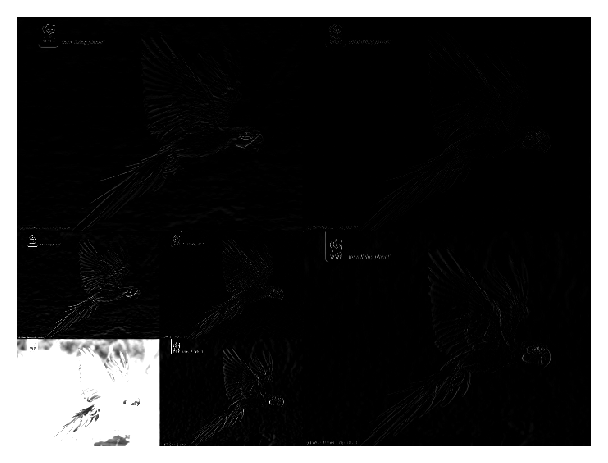
\includegraphics[width = 0.5 \linewidth]{ara_sqrt2.eps} &
	  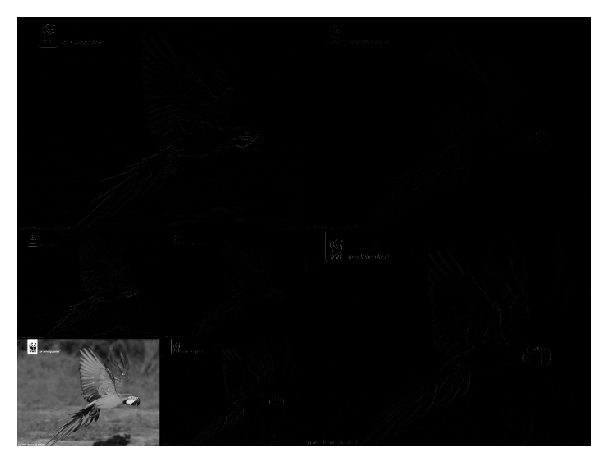
\includegraphics[width = 0.5 \linewidth]{ara_wt_V1.eps} \\	
	  
	\end{tabular}
	
	\caption{Exemple de la diff\'{e}rence entre le choix du scalaire $\frac{1}{\sqrt{2}}$ (\`{a} gauche) 
	    et du scalaire $\frac{1}{2}$ (\`{a} droite)}
	
      \end{figure}   
    \end{frame}
    
    \begin{frame}
      \centering
      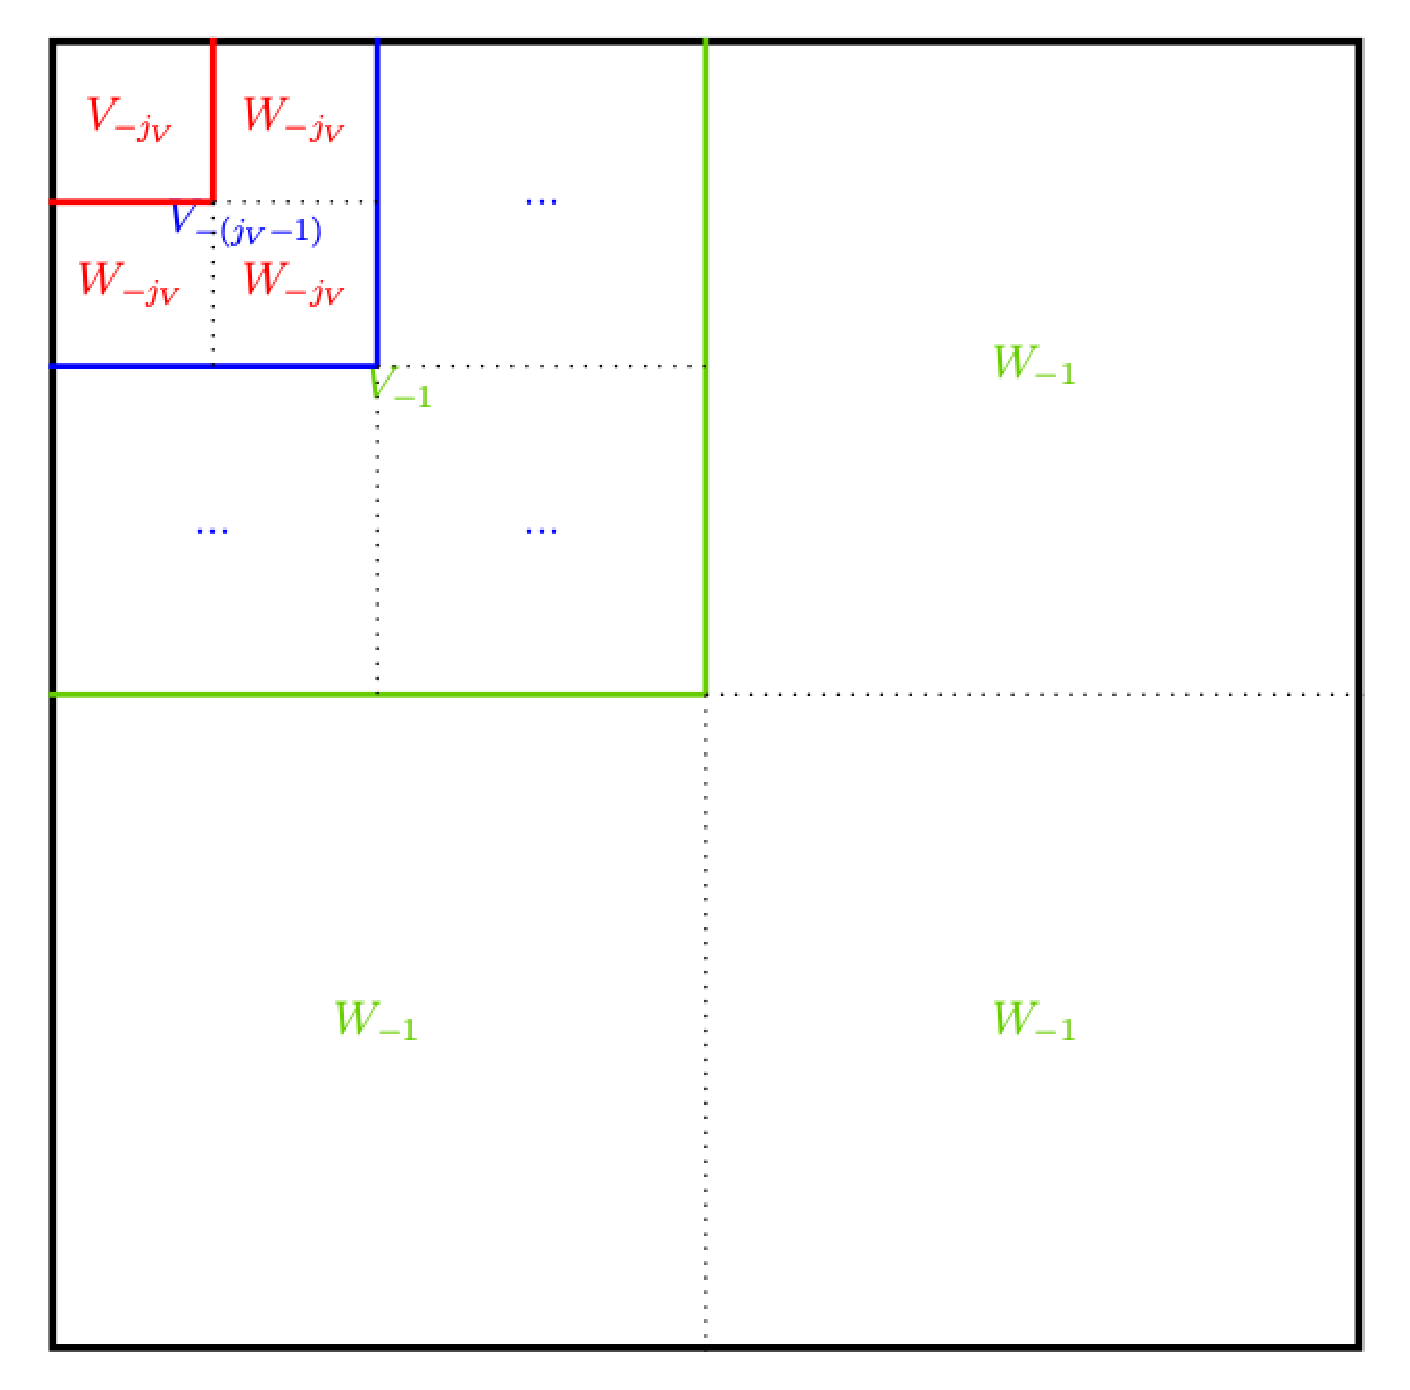
\includegraphics[width = 0.7 \linewidth]{detail.eps}
    \end{frame}
    
    \begin{frame}
     \begin{figure}[!h]
	\centering
	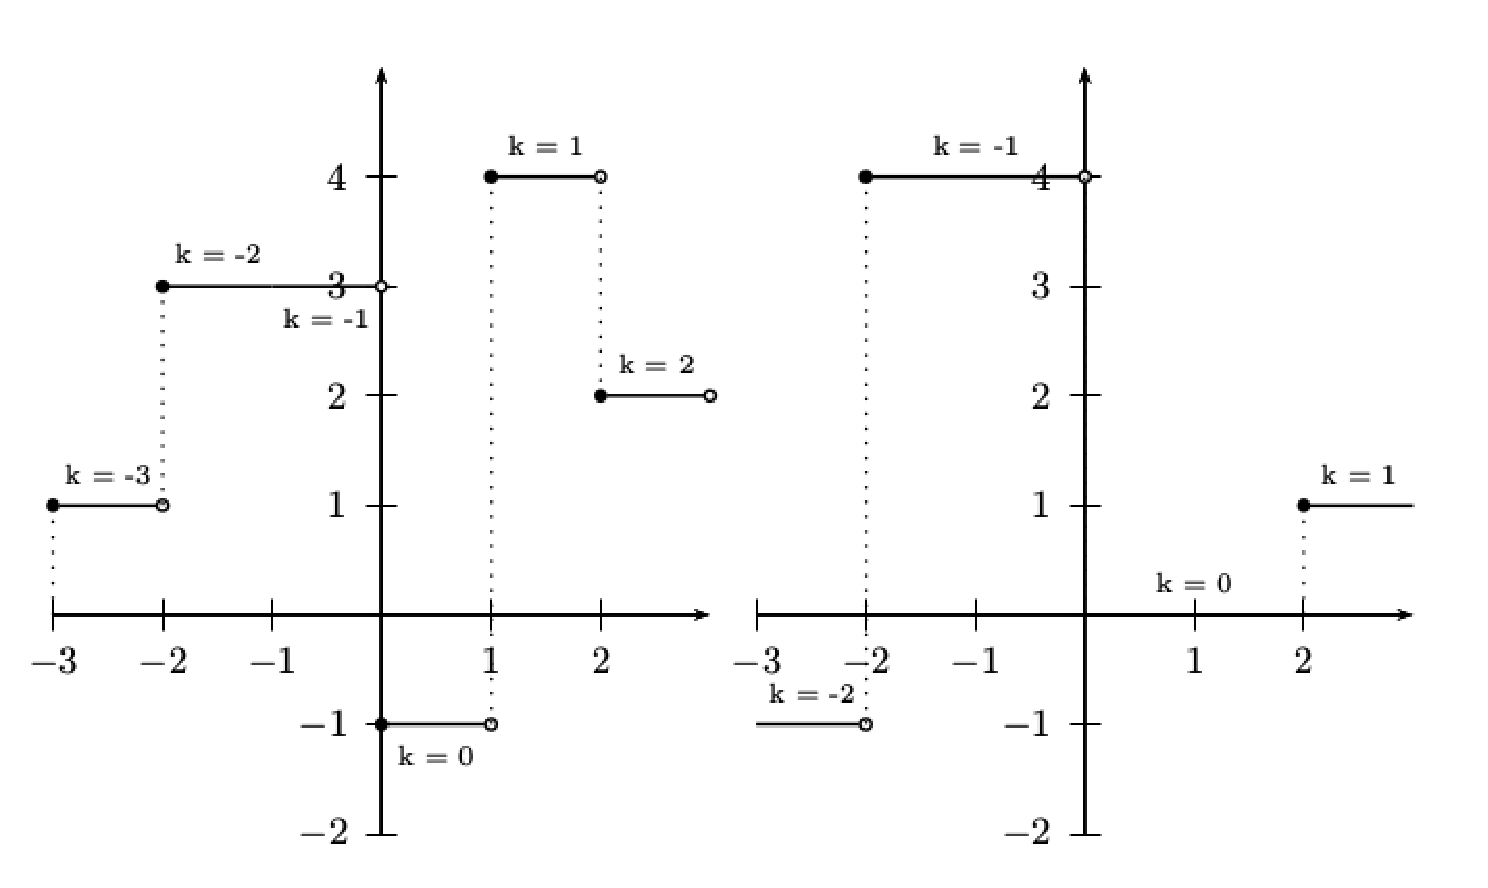
\includegraphics[width = 0.7 \linewidth]{espaces.eps}
	\caption{Exemple graphique d'une fonction de $V_0$ (\`{a} gauche) et de $V_1$ (\`{a} droite)}
      \end{figure}
    \end{frame}

    
    \begin{frame}[allowframebreaks]
      \frametitle{D\'{e}monstration de la densit\'{e}}
	  Soit $\varepsilon \, > \, 0$. Soit $f \, \in \, L^2(\mathbb{R},\mathbb{R})$ telle que $f$ est continue par morceaux un nombre fini de fois
	  et de support compact et admettant une limite (nulle).\\
	  $f$ est continue par morceaux sur des intervalles que l'on va noter $(D_n)_{n \in I}$ avec $I \subset \mathbb{N} $, $I$ fini. \\
	  On va donc limiter l'\'{e}tude \`{a} un intervalle $D_n$ pour $n \in I$. \\
	  On pose $D_n \, = \, ]\alpha; \beta[$. \\
	      
	  \underline{Cas 1 : $\alpha \neq - \infty$ et $\beta \neq + \infty$} \\
	  $\phantom{Prop}$ Ainsi la fonction $f$ est prolongeable par continuit\'{e} sur $\overline{D_n} \, = \, [\alpha; \beta]$. \\
	  $\phantom{Prop}$ Par cons\'{e}quent, $f$ est continue sur un segment donc, par th\'{e}or\`{e}me de Heine, elle y est uniform\'{e}ment continue. \\
	  $\phantom{Prop}$ Par d\'{e}finition de continuit\'{e} uniforme, on a :
	  \begin{center}
	    $\exists \delta_n > 0, \forall x, y \in D_n, \mid x - y \mid \, \leqslant \delta_n \; \Rightarrow \; \mid f(x) - f(y) \mid \, \leqslant \varepsilon$
	  \end{center}

	  $\phantom{Prop}$ Or, d'autre part, $\displaystyle \lim_{j \rightarrow - \infty} 2^j \; = \; 0$ et 
		$\displaystyle \lim_{j \rightarrow + \infty} 2^j \; = \; + \infty$ donc \\ 
	  $\phantom{PropPropProp}$ $ \exists j_n \in \mathbb{Z}, 2^{j_n} \leqslant \delta_n < 2^{j_n + 1} $
	  
	  $\phantom{Prop}$ Ainsi $\forall x, y \in D_n, \mid x - y \mid \, \leqslant 2^{j_n} \; \Rightarrow \; \mid f(x) - f(y) \mid \, \leqslant \, \varepsilon $. \\
	  
	  \underline{Cas 2 : $\alpha \neq - \infty$ ou $\beta \neq + \infty$} \\
	  $\phantom{Prop}$ Dans ce cas, on proc\'{e}de de m\^{e}me en se ramenant \`{a} un segment en utilisant la d\'{e}finition de la 
	      limite appliqu\'{e}e \`{a} $\varepsilon$ en $\pm \infty$. \\
	  
	  $\phantom{Prop}$ Dans tous les cas, on pose alors une fonction $ \psi_n \in V_{j_n} $ telle que pour tout intervalle de la forme $[2^{j_n} k; 2^{j_n} (k + 1)[$ o\`{u} $k \in \mathbb{Z}$,
	  il existe un $x_{n,k} \in J_n$ tel que $ \forall y \in [2^{j_n} k; 2^{j_n} (k + 1)[, \, \psi_n (y) \; = \; f(x_{n,k})$ 
	  (ce $x_{n,k}$ existe sous condition que $ [2^{j_n} k; 2^{j_n} (k + 1)[ \; \subset \; D_n $, si ce n'est pas le cas,
	  on pose alors $ \psi_n \mid_{[2^{j_n} k; 2^{j_n} (k + 1)[} \; = \; 0$). \\
	  
	  On obtient donc un ensemble d'indices $J_n \; = \; \Big\{ j_n, n \in I \Big\}$
	  et un ensemble de fonctions $\Big\{ \psi_n , n \in I \Big\} \; \subset \; \displaystyle \bigcup_{j \in \mathbb{Z}} V_j $. \\
	  
	  Par propri\'{e}t\'{e} d'inclusion $(i)$, en posant $j_{\varepsilon} \; = \; \min J_n$ (existe car $I$ est fini),
	  et en d\'{e}finissant $P_{V_{j_{\varepsilon}}}$ \`{a} l'aide des $\psi_n$ pour $n \in I$, on obtient que :
	  
	  \begin{center}
	    $ \boxed{\displaystyle \bigcup_{j \in \mathbb{Z}} V_j $ est dense dans $ L^2(\mathbb{R}, \mathbb{R})} $  $\blacksquare$
	  \end{center}
    \end{frame}
    
    \begin{frame}
      \frametitle{D\'{e}monstration de la complexit\'{e}}
      
	Soit $j_V \in \mathbb{N}$. Soit $M \in M_{n,m}(\mathbb{R})$. \\
	La complexit\'{e} de la normalisation est de l'ordre de $O (nm) $. \\
	Soit $k \in [0; j_v - 1]$. Soit $i \in [1;n/2^k]$ \\
	Comme la complexit\'{e} de l'affectation est lin\'{e}aire en la taille du vecteur,
	l'affectation a une complexit\'{e} de $ \frac{m}{2^{k+1}}$.\\
	De plus, la fonction $ \downarrow_2 \; $o$ \; \varPhi $ s'effectue en un temps quadratique en la taille du vecteur 
	(due \`{a} la fonction filtre).\\
	Ainsi, le calcul du r\'{e}sultat de cette fonction appliqu\'{e} au vecteur $M_{i, [1;\frac{m}{2^k}]}$ a une 
	complexit\'{e} de $C (\frac{m}{2^k})^2$ avec $C > 0$. \\

	Ainsi, la premi\`{e}re boucle s'effectue en $ O \Big(\frac{n m^2}{2^{3k - 1}} \Big) $. \\
	On d\'{e}montre de m\^{e}me que la deuxi\`{e}me boucle s'effectue en $ O \Big(\frac{m n^2}{2^{3k - 1}} \Big) $. \\
	
	Ainsi la complexit\'{e} de cet algorithme est bien de \\
	$ \boxed{O \Big(nm + n m^2 + m n^2 \Big)} $  $\blacksquare$
    \end{frame}

    \begin{frame}
      \frametitle{D\'{e}monstration de $(WR)$o$(WT) \; = \; id$}
      
      Soit $(x, y) \in \mathbb{R}^2$.
      Par d\'{e}finition des algorithmes, il s'agit en fait de d\'{e}montrer que :
      
      \begin{center}
	$ \Phi_{1, \mathcal{R}_a} \Big(\Phi_{1, \mathcal{H}_a}(x, y), \Phi_{1, \mathcal{H}_d}(x, y) \Big) \; = \; x $ \\
	$ \Phi_{1, \mathcal{R}_d} \Big(\Phi_{1, \mathcal{H}_a}(x, y), \Phi_{1, \mathcal{H}_d}(x, y) \Big) \; = \; y $
      \end{center}
      
      C'est \`{a} dire, par d\'{e}finition des fonctions filtres, qu'il s'agit de montrer que :
      
      \begin{center}
	$ \frac{x + y}{2} + \frac{x - y}{2} \; = \; x $ \\
	$ \frac{x + y}{2} - \frac{x - y}{2} \; = \; y $
      \end{center}
      
      Ce qui est clairement le cas  $\blacksquare$
    \end{frame}
    
\end{document}
